% !TeX encoding = UTF-8
% !TeX spellcheck = en_US
% !TeX program = xelatex
\documentclass[11pt, a4paper]{article}

\usepackage{amsmath}

% ---------- CHOOSE A FONT ----------

%\usepackage{fontspec}
%\setmainfont{Raleway}

\usepackage[OT1]{fontenc}
\usepackage[math]{iwona}

\usepackage[english]{babel}						   % hyphenation etc for English
\usepackage{csquotes}

% --------- MISC FORMATTING ---------
%
\usepackage{setspace}                % needed for doublespacing
%\doublespacing                       % doublespaced line spacing
\usepackage{graphicx}                % for importing graphics into figures
\usepackage{float}					 % better control of figure placement
\usepackage[hyphens]{url}                 
\usepackage{hyperref}                % for clickable URLs and email addresses
\usepackage{cleveref}
\urlstyle{sf}                        % sans-serif font for URLs
\usepackage[margin=1.2in]{geometry}  % control page margins
\usepackage[labelfont=bf]{caption}   % make caption labels boldface
\usepackage[bottom]{footmisc}        % footnotes at bottom of page
\setlength{\skip\footins}{10mm}      % obsessing about footnote spacing
\setlength{\parskip}{1ex}            % space between paragraphs
%\setlength{\parindent}{3em}	     % paragraph indentation
\usepackage{authblk}                 % author and affiliation formatting
\renewcommand\Affilfont{\small}
\usepackage{booktabs}
\usepackage{multirow}
\usepackage{pdflscape}
\usepackage[table]{xcolor}
\usepackage{easyReview}

%\setlength\overfullrule{5pt}

% Biblio
\usepackage[style=apa,
labeldate=year,
isbn=false,
eprint=false,
date=year,
url=false,
backend=biber]{biblatex}
\bibliography{references.bib}

%-----------
% Line numbers
\usepackage{lineno}                  % add line numbers to margin
\def\linenumberfont{\normalfont\footnotesize\sffamily} % line numbers
\setlength\linenumbersep{9mm}                          % line numbers
\linenumbers                                           % line numbers


%-----------
\usepackage[section]{placeins}


\title{Draft genomes of the three northern hemisphere blue mussel lineages: North and South European \emph{Mytilus edulis} and Mediterranean \emph{Mytilus galloprovincialis}.}

\author[1,*]{Alexis Simon}
\author[1]{Christine Arbiol}
\author[1]{Nicolas Bierne}

\affil[1]{CNRS, Univ Montpellier, \ldots{}}

%

\begin{document}

\maketitle


\vspace{1cm}
\hrule
\begin{abstract}
	Using the 10X chromium long reads technology, we provide draft genomes for three closely related blue mussel species from the \emph{Mytilus} species complex.
	The objective was to produce affordable genomic resources for population and evolutionary genomic studies.
	Genomes are fragmented but represent a large portion of the genome, with good sizes and BUSCO scores.
\end{abstract}

\vspace{3mm}
\hrule
\vspace{5mm}

\noindent
\textbf{Keywords}: \emph{Mytilus edulis}, \emph{Mytilus galloprovincialis}, Genome assembly, 10X chromium

\noindent
$^{*}$ \textbf{Corresponding author}: \href{mailto:alexis.simon@normalesup.org}{\nolinkurl{alexis.simon@normalesup.org}}

\newpage

\section{Rationale and objectives}\label{introduction}

The \textit{Mytilus} species complex has been a model system in population genetics, adaptation, hybridization and speciation since genetic variants could be identified \parencite{Milkman1970, Koehn1972, Ahmad1977, Skibinski1978, Quesada1995b, Bierne2003, Fraisse2016a, Simon2021}.

The \textit{Mytilus} species complex is composed of three taxonomically recognized and partially reproductively isolated species in the northern hemisphere,
\textit{Mytilus edulis}, \textit{M. galloprovincialis} and \textit{M. trossulus}.
Within each species, evolutionary relevant lineages can be identified.
Two lineages of \textit{M. galloprovincialis} can be identified, one Atlantic lineage and one Mediterranean lineage separated by a hybrid zone along the Almeria-Oran front \parencite{Quesada1995, Fraisse2016a, ElAyari2019}.
Three lineages of \textit{M. edulis} can be identified: (i) an American lineage, (ii) a Southern European lineage, and (iii) a Northern European lineage \parencite{Fraisse2016a, Simon2020}.

As an effort to diversify the genomic resources available for the \textit{Mytilus} species complex,
we assembled and annotate the genomes of three lineages using the 10X chromium technology.
While our assemblies were initially fragmented due to the high level of heterozygosity,
we leveraged the existence of a chromosome scale assembly of a sister species to scaffold our assemblies against it.
We obtained assemblies equivalent to published ones in term of completeness for three new lineages of the species complex using a low sequencing budget and publicly available data.
The resources produced and the assembly pipeline are freely available for use by the community.

\section{Methods}\label{methods}

\paragraph{General notes:}
The entire assembly was carried out using a Snakemake \parencite{Molder2021} pipeline available on github at \url{https://github.com/alxsimon/assembly_10x}.
Where deemed important, parameters are given in the text.
For brevity and simplicity, not all information might be available in the text.
However, all parameters, software versions and steps are retrievable from the repository.

\paragraph{Important caveat:}
The assembled genome of MeduEUN (\textit{M. edulis} Northern lineage) was initially thought to be \textit{M. trossulus}.
Therefore some assembly and annotation steps wrongly used \textit{M. trossulus} transcriptomes.
While this is not ideal, we think results have not been strongly impacted by this issue.


\subsection{Biological material and DNA extraction}

One individual for each species of interest was collected and processed fresh.

Collection locations:
\begin{itemize}
	\item \emph{M. galloprovincialis} Mediterranean MgalMED; Sète, France
	\item \emph{M. edulis} Southern European MeduEUS; ???
	\item \emph{M. edulis} Northern Europe MeduEUN; ???
\end{itemize}

Whole mussels were placed in 50 mL falcon tubes containing 25 ml of TNES-Urea solution and incubated for 4-6 weeks at room temperature (TNES-Urea: 10 mM Tris-HCl pH 7.4; 120 mM NaCl; 10 mM EDTA pH 8.0; 0.5\% SDS; 4 M urea).

After this period of pre-treatment at ambient temperature, proteinase K was added at a final concentration of 150 \(\mu\)g/mL and the solution was incubated overnight at 56°C.

High Molecular weight genomic DNA was extracted following \textcite{Nakayama1994}.
We used a 15 mL Phase Lock Gel Heavy extraction with 3 steps of phenol/chloroform/isoamylalcool (25/24/1) Tris pH 8,1 followed by 2 chloroform extractions.
After the last extraction, the aqueous supernatant was precipitated with 2 volumes of 100\% EtOH and the pellet was hooked from the solution with a sterile glass Pasteur pipette.
The pellet was rinsed several times in 80\% EtOH before being dried at room temperature.

DNA was resuspended with an appropriate volume of biomolecular water at 65°C for several hours, the duration of this incubation depending on the size of the granules.
DNA was then stored at 4°C.

Prior to the construction of the DNA libraries, DNA was repaired with NEBNext FFPE DNA Repair Mix according to the manufacturer's instructions.


\subsection{Library preparation and sequencing}

The 10X chromium library preparation and sequencing was subcontracted to the MGX platform (Montpellier, France).
The 10X linked reads libraries for each individual were produced following the 10X Genomics Genome Reagen Kit (\emph{Genome Solution}) protocol using a Chromium microfluidic chip.
Libraries were subsequently sequenced on an Illumina NovaSeq 6000 with an S4 flowcell.

\subsection{Preprocessing 10X reads}\label{preproc}

We preprocessed 10X reads using the following pipeline for use in several algorithms (\cref{draft_asm}).
We first removed duplicate reads using \texttt{Nubeam-dedup} (\cite{Dai2020}; commit 25dd385).
We then used \texttt{proc10xG} (\url{https://github.com/ucdavis-bioinformatics/proc10xG}; commit 7afbfcf) to split the reads from their 10X barcodes for further processing.
We used a custom filtering step designed to remove under- and over-represented barcodes and their associated reads from the data (\cref{supfig:preproc_MgalMED,supfig:preproc_MeduEUS,supfig:preproc_MeduEUN}, \texttt{filter\_barcodes.R} script, see \cite{Bary\&Gagnaire??}).
[[Add supfigs of filter\_barcodes]].
Reads were additionally filtered with \texttt{fastp} (v0.20.1; \cite{Chen2018}) with the main objective to remove poly-G tails created by the Illumina Novaseq sequencing technology.
We obtained at this point reads equivalent to a short-read sequencing run, usable in some parts of the assembly and quality control pipeline.
Additionally, to obtain reads compatible to 10X genomics tools, we filtered and reassembled reads with their 10X barcodes in \texttt{proc10xG} using the \texttt{filter\_10xReads.py} and \texttt{regen\_10xReads.py} scripts.

\subsection{Initial genome assemblies}\label{draft_asm}

For each genome we used \texttt{Supernova} v2.1.1 \parencite{Weisenfeld2017} to assemble raw 10X reads.
To avoid hard stops in \texttt{Supernova} due to both data quantity slightly under 10X genomics recommendations and an overestimation of genome size by Supernova, we used all available reads (\texttt{--maxreads='all'}) and accepted extreme coverage (\texttt{--accept-extreme-coverage}).
We produced every style of Fasta output available in \texttt{Supernova} but only used the pseudo-haploid output in the following pipeline.

To remove duplicate haplotypes in the assemblies, we followed the \texttt{purge\_dups} pipeline (\cite{Guan2020}; commit e1934bb).
We first used the \texttt{longranger} v2.2.2 align algorithm to map preprocessed reads (\cref{preproc}) to the pseudo-haploid genomes to use in the \texttt{ngscstat} step.
\texttt{Minimap2} (v2.17; \cite{Li2017}) was used in the contig self-mapping step.
We obtained the purged assemblies using the \texttt{get\_seqs} steps without restricting the purging to the end of contigs (without the \texttt{-e} option).

We used \texttt{AGOUTI} (\url{https://github.com/svm-zhang/AGOUTI}; commit a7e65d6; \cite{Zhang2016a}) to improve scaffolding by using paired end RNA-seq reads.
For each species, a different set of published transcriptomes were used (Supplementary Table [[...]] for accessions).
\texttt{AGOUTI} require a gene prediction as input in addition to RNA-seq reads.
We used \texttt{Augustus} (v3.3.3; \cite{Stanke2008}) to produce an intermediate annotation for each assembly using the \textit{Caenorhabditis} model.
RNA-seq reads were first cleaned using \texttt{rcorrector} (v1.0.4; \cite{Song2015}) and \texttt{trimgalore} (v0.6.6; \url{https://www.bioinformatics.babraham.ac.uk/projects/trim_galore}; \texttt{--quality 20 --stringency 1 -e 0.1 --length 70}).
RNA-seq reads were mapped independently using \texttt{bwa-mem2} (v2.2.1; \cite{VasimuddinMd2019}), and then merged as a common bam file for each assembly with \texttt{samtools} (v1.12; \cite{Li2009}).
Finally, the \texttt{AGOUTI} scaffolding pipeline was run using the gene prediction and mapped RNA-seq reads (-minMQ 20 -maxFracMM 0.05; using \texttt{python} v2.7.15 and \texttt{samtools} v1.10 for compatibility).

As a last step, we ran \textit{Blobtoolkit} (v2.4.0; \cite{Challis2020}) on the three assemblies to evaluate quality and potential contamination levels.
We used a custom script (\texttt{btk\_conta\_extraction.py}) to filter the assembly contigs based on the taxids found by the \textit{Blobtoolkit} pipeline to remove the most obvious contaminations.
Contigs matching taxids associated with viruses, bacteria and non-mollusca eukaryotes were removed.
More specifically contigs for were removed for virus contamination if they presented a hit percentage of more than 10~\% of their length.
Contigs were removed for eukaryote contamination only when presenting only hits to taxa outside Mollusca on more than 10~\% of their length.
The list of retained contigs was used to filter the fasta assembly file using \texttt{seqkit} (v0.13.2; \cite{Shen2016}).


\subsection{Scaffolding on the \textit{Mytilus coruscus} genome}

At the time of assembly, the closest relative of the \textit{Mytilus} species of interest with a chromosome scale assembly was \textit{Mytilus coruscus} (GCA\_017311375.1; \cite{Yang2021}).
Given the conserved number of 14 chromosomes in the \textit{Mytilus} genus, we decided to scaffold our contigs on this high quality reference.
Additionally, we had Oxford Nanopore reads for the MeduEUN individual. 
We used \texttt{minimap2} (v2.17; \cite{Li2017}) and \texttt{LRScaf} (v1.1.10; \url{https://github.com/shingocat/lrscaf}) to first improve the MeduEUN assembly with this small amount of long reads.

Then for each assembly, we ran the scaffolder \texttt{RagTag} (v1.1.1; \cite{Alonge2021}) to position contigs on the \emph{M. coruscus} chromosomal assembly.

A final polishing step was performed using \texttt{Pilon} (v1.24; \cite{Walker2014}).
\texttt{Pilon} attempts to improve the assembly based on mapped read information (gap filling and error corrections).
We used \texttt{bwa-mem2} to map the debarcoded and filtered 10X reads (\cref{preproc}).
In addition, Oxford Nanopore reads for MeduEUN were also used in \texttt{Pilon} for the given assembly.

\subsection{Repeats}

We masked repeats for the purpose of annotation using \texttt{RepeatModeler} (v2.0.1; \cite{Flynn2020}) and \texttt{RepeatMasker} (v4.1.2-p1; \cite{Smit2013}) through the TETools DFAM container (v1.3.1; \url{https://hub.docker.com/r/dfam/tetools}).
We first built repeat databases for each of five assemblies MgalMED, MeduEUS, MeduEUN, \textit{M. coruscus} (GCA\_017311375.1; \cite{Yang2021}) and \textit{M. galloprovincialis} from the Atlantic (GCA\_900618805.1; \cite{Gerdol2020}).
Then, we built a common \textit{Mytilus} database of repeats by merging those five databases using \texttt{cd-hit} (v4.8.1; \cite{Fu2012}). We used the same options as used by default in \texttt{RepeatModeler}: \texttt{-aS 0.8 -c 0.8 -g 1 -G 0 -A 80 -M 10000}.
Finally, soft repeat masking was performed on the assemblies with \texttt{RepeatMasker} using the merged database.

\subsection{Annotation}

To obtain an annotation for each assembly, we used both database and RNA-seq information.
We used \texttt{Braker2} (v2.1.6; \cite{Bruna2021}) as an initial step, using both a protein database and RNA-seq reads (preprocessed in \cref{draft_asm}).
To build the protein database, we used all \textit{Mollusca} proteins (taxid 6447) from OrthoDB (v10.1; \cite{Kriventseva2019}).
To provide gene presence hints, we mapped all RNA-seq reads for each species using \texttt{HISAT2} (v2.2.1; \cite{Kim2019}).

We used the \texttt{Mantis} pipeline (\url{https://github.com/PedroMTQ/mantis}; commit c6cb597; \cite{Queiros2021}) to obtain consensus annotations of genes based on multiple databases.
Protein sequences for each assembly were built from the \texttt{Braker2} annotation using the \texttt{python} module \texttt{gff3tool} (v2).

\subsection{NCBI submission}

The NCBI submission process identified a few errors that needed correcting.
A small number of adaptor sequences and duplicates were removed to comply with NCBI requirements
(see the rule \texttt{ncbi\_submission\_changes.smk} in the pipeline for more details).
Assemblies are available under the following accessions: 
JAKGDF000000000 for MgalMED,
JAKGDG000000000 for MeduEUS,
and JAKGDH000000000 for MeduEUN.


\subsection{Quality assessments and comparisons}

Preprocessed 10X reads (\cref{preproc}) were used to first estimate estimate genome size and heterozygosities of the three individuals.
We used the reference free k-mer based method \texttt{GenomeScope} (\url{https://github.com/tbenavi1/genomescope2.0}; commit 5034ed4; \cite{Ranallo-Benavidez2020}) and the fork of the \texttt{KMC} k-mer  counting program (\url{https://github.com/tbenavi1/KMC}; commit 1df71f6).

Assembly statistics were computed with the python module \texttt{assembly\_stats} (v0.1.4; \cite{Trizna2020}).

To assess the remaining level of duplication in the assemblies, we used the program \texttt{KAT} (v2.4.2; \cite{Mapleson2017}) to compare k-mer spectra from reads (preprocessed 10X) and from the assembly.

Finally, gene completion analyses were carried out using \texttt{BUSCO} (v5.1.1; \cite{Manni2021}).
We used both a Metazoan (\texttt{metazoa\_odb10.2021-02-24}) and Molluscan (\texttt{mollusca\_odb10.2020-08-05}) database to assess and compare new and published assemblies.
We compared our assemblies to the following published ones:
\begin{itemize}
	\item \textit{M. coruscus}, GCA\_017311375.1, \textcite{Yang2021};
	\item \textit{M. galloprovincialis} from the Altantic lineage, GCA\_900618805.1, \textcite{Gerdol2020};
	\item \textit{M. edulis} from the Southern European lineage, GCA\_905397895.1, \textcite{Corrochano-Fraile2021}
	\item \textit{M. edulis} from the American lineage, GCA\_019925275.1.
\end{itemize}


\subsection{Phylogenetic species tree}

We compiled protein sequences from published \textit{Mytilus} genomes and transcriptomes,
in addition to the current three genomes and annotations, to build a species tree.
We used transcriptomes produced in \textcite{Popovic2020a} for American \textit{M. edulis}, 
Mediterranean \textit{M. galloprovincialis}, \textit{M. trossulus}, \textit{M. californianus}.
Transcriptomes were translated using the \texttt{seqkit} program (v2.2.0; \cite{Shen2016})
We used genomes and associated annotations of \textit{M. coruscus} (GCA\_017311375.1; \textcite{Yang2021}),
Southern European \textit{M. edulis} (GCA\_905397895.1; \textcite{Corrochano-Fraile2021}),
Atlantic \textit{M. galloprovincialis} (GCA\_900618805.1; \textcite{Gerdol2020}),
and American \textit{M. edulis} (GCA\_019925275.1; annotation as personal communication of Tiago Hori, PEIMSO).
For GCA\_019925275.1, protein sequences where retrieve from the fasta and gff files using the python module gff3tool (v2.1.0).

We used \texttt{Orthofinder} (v2.5.2; \cite{Emms2015, Emms2019}) to find orthogroups and orthologue genes.
Species tree was inferred using the MSA method of \texttt{Orthofinder} \parencite{Emms2018} and \texttt{IQTREE} (v2.2.0\_beta; \cite{Minh2020}) tree inference.

%\begin{itemize}
%	\item Supernova v2.1.1 \href{https://doi.org/10.1101/gr.214874.116}{cite}
%	\item Longranger v2.2.2
%	\item proc10xG \url{https://github.com/ucdavis-bioinformatics/proc10xG} commit 7afbfcf
%	\item nubeam-dedup \url{https://github.com/daihang16/nubeamdedup} commit 25dd385 \href{https://doi.org/10.1093/bioinformatics/btaa112}{cite}
%	\item KMC \url{https://github.com/tbenavi1/KMC} commit 1df71f6
%	\item GenomeScope 2.0 \url{https://github.com/tbenavi1/genomescope2.0} commit 5034ed4 \href{https://doi.org/10.1038/s41467-020-14998-3}{cite}
%	\item (? Smudgeplot commit 950d7b5)
%	\item Purge\_Dups \url{https://github.com/dfguan/purge_dups} commit e1934bb \href{https://doi.org/10.1093/bioinformatics/btaa025}{cite}
%	\item AGOUTI \url{https://github.com/svm-zhang/AGOUTI} commit a7e65d6 \href{https://doi.org/10.1186/s13742-016-0136-3}{cite}
%	\item augustus v3.3.3 (for AGOUTI analysis) (\protect\hyperlink{ref-Stanke2008}{\textbf{Stanke2008?}})
%	\item Blobtoolkit v2.4.0 \href{https://doi.org/10.1534/g3.119.400908}{cite}
%	\item KAT v2.4.2 \href{https://doi.org/10.1093/bioinformatics/btw663}{cite}
%	\item fastp v0.20.1 (\protect\hyperlink{ref-Chen2018a}{\textbf{Chen2018a?}})
%	\item samtools v1.12 (\protect\hyperlink{ref-Li2009}{\textbf{Li2009?}})
%	\item minimap2 v2.17 (\protect\hyperlink{ref-LiLi2017}{\textbf{LiLi2017?}})
%	\item bwa-mem2 v2.2.1 (\protect\hyperlink{ref-VasimuddinMd2019}{\textbf{VasimuddinMd2019?}})
%	\item bedtools v2.29.2 (\protect\hyperlink{ref-Quinlan2010}{\textbf{Quinlan2010?}})
%	\item seqkit v0.13.2 (\protect\hyperlink{ref-Shen2016}{\textbf{Shen2016?}})
%	\item rcorrector v1.0.4
%	\item trim-galore v0.6.6 \href{https://github.com/FelixKrueger/TrimGalore}{cite} (Cutadapt + FastQC wrapper)
%	\item busco v5.1.1 (\protect\hyperlink{ref-Seppey2019}{\textbf{Seppey2019?}})
%	\item assembly\_stats v0.1.4 \href{https://doi.org/10.5281/zenodo.3968774}{cite}
%	\item ragtag v1.1.1 (\protect\hyperlink{ref-Alonge2019}{\textbf{Alonge2019?}})
%	\item pilon v1.24 (\protect\hyperlink{ref-Walker2014}{\textbf{Walker2014?}})
%	\item TETools DFAM container v1.3.1
%	\item RepeatModeler v2.0.1 (\protect\hyperlink{ref-Flynn2020}{\textbf{Flynn2020?}})
%	\item cd-hit v4.8.1 (\protect\hyperlink{ref-Fu2012}{\textbf{Fu2012?}})
%	\item RepeatMasker v4.1.2-p1 (Smit, AFA, Hubley, R. RepeatModeler Open-1.0. 2008-2015 \url{http://www.repeatmasker.org}) (\protect\hyperlink{ref-Smit2013}{\textbf{Smit2013?}})
%\end{itemize}


\section{Results and discussion}

The pre-assembly k-mer analysis carried out using GenomeScope (using 21-mers) showed that, as expected, the genomes were highly heterozygous with values going from 3.49 to 8.77~\% (\cref{fig:genomescope}).
GenomeScope provide a bad fit and estimation in the case of the MeduEUS data due to a reduced coverage of the genome in that case, compared to the two other assemblies.

Highly heterozygous genomes brings the risk of having a large number of duplicate contigs due to the separate assembly of the two alleles from a same locus.
For this reason, we used the \texttt{purge\_dups} pipeline to try removing a maximum of such bias.
This procedure reduced the number of complete duplicated genes in all assemblies (\cref{supfig:busco}, v1 to v4).

\begin{figure}[h]
	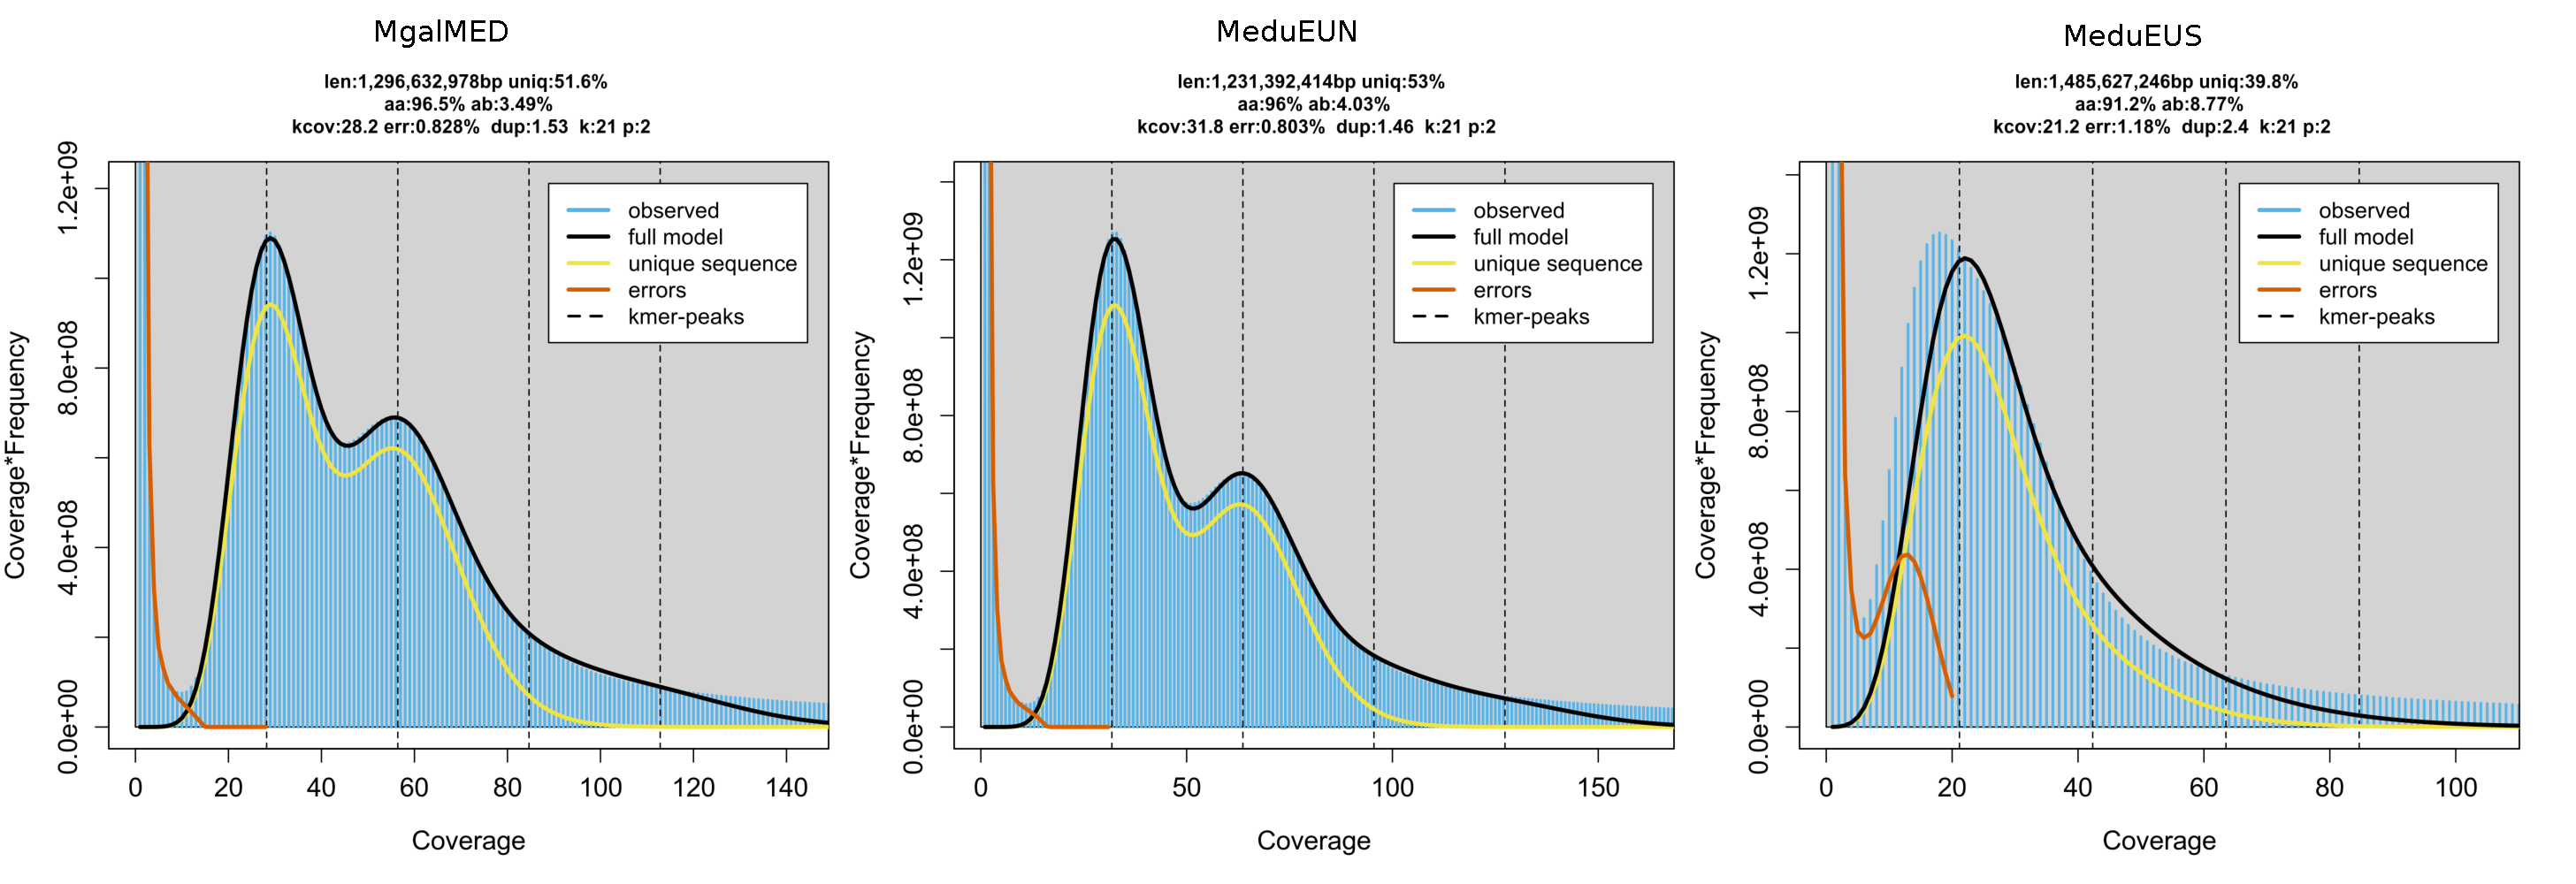
\includegraphics[width=\linewidth]{figures/Fig1_genomescope.pdf}
	\caption{k-mer profile plots computed with 21-mers using GenomeScope.
		Coverage histogram of the k-mers in blue.
		Lines represent the fit of the GenomeScope models.
		len: inferred genome length; uniq: percentage of the genome that is unique, aa: overall homozigosity; ab: overall heterozygosity; kcov: mean k-mer coverage for heterozygous bases; err: reads error rate; dup: average rate of read duplication; k: k-mer size; p: ploidy.
	}
	\label{fig:genomescope}
\end{figure}

% Table 1
\begin{landscape}
	% latex table generated in R 4.1.2 by xtable 1.8-4 package
% Thu Jan 20 14:13:47 2022
\begin{table}[ht]
\centering
\caption{
Assembly statistics comparisons. C for contigs and S for scaffolds.
} 
\label{tab:asm_stats}
\scalebox{0.7}{
\begin{tabular}{lrrrrrrrrrr}
  \toprule
assembly & C.L50 & C.N50 & C.median & C.sequence\_count & S.L50 & S.N50 & S.gc\_content & S.median & S.sequence\_count & S.total\_bps \\ 
  \midrule
Mcor\_GCA017311375 & 261 & 1481111 & 42077 & 6449 & 6 & 99542347 & 32.4 & 21293 & 4434 & 1566529938 \\ 
  MgalATL\_GCA900618805 & 4922 & 77035 & 39489 & 22922 & 1903 & 207642 & 32.1 & 77568 & 10577 & 1282208009 \\ 
  MeduEUS\_GCA905397895 & 977 & 511485 & 184638 & 5966 & 464 & 1097279 & 32.2 & 292104 & 3339 & 1827085763 \\ 
  MeduAM\_GCA019925415 & 835 & 490737 & 62522 & 9686 & 6 & 116503180 & 32.3 & 28931 & 1119 & 1651313236 \\ 
  MgalMED\_v7 & 16906 & 26323 & 7475 & 115913 & 9 & 71952646 & 32.1 & 4531 & 41122 & 1658656017 \\ 
  MeduEUS\_v7 & 24467 & 23624 & 6478 & 169324 & 415 & 228263 & 34.6 & 4999 & 73616 & 2076685641 \\ 
  MeduEUN\_v7 & 15862 & 29157 & 8961 & 105892 & 9 & 77102752 & 32.1 & 6164 & 28220 & 1764246486 \\ 
   \bottomrule
\end{tabular}
}
\end{table}

\end{landscape}


To assess the completeness of our assemblies, we compared them to four \textit{Mytilus} published assemblies on the basis of a Metazoan and a Molluscan set of single copy orthologous genes using BUSCO (\cref{fig:busco}).
Overall, we show that our assemblies are equivalent to the published ones in terms of completeness.

\begin{figure}[h]
	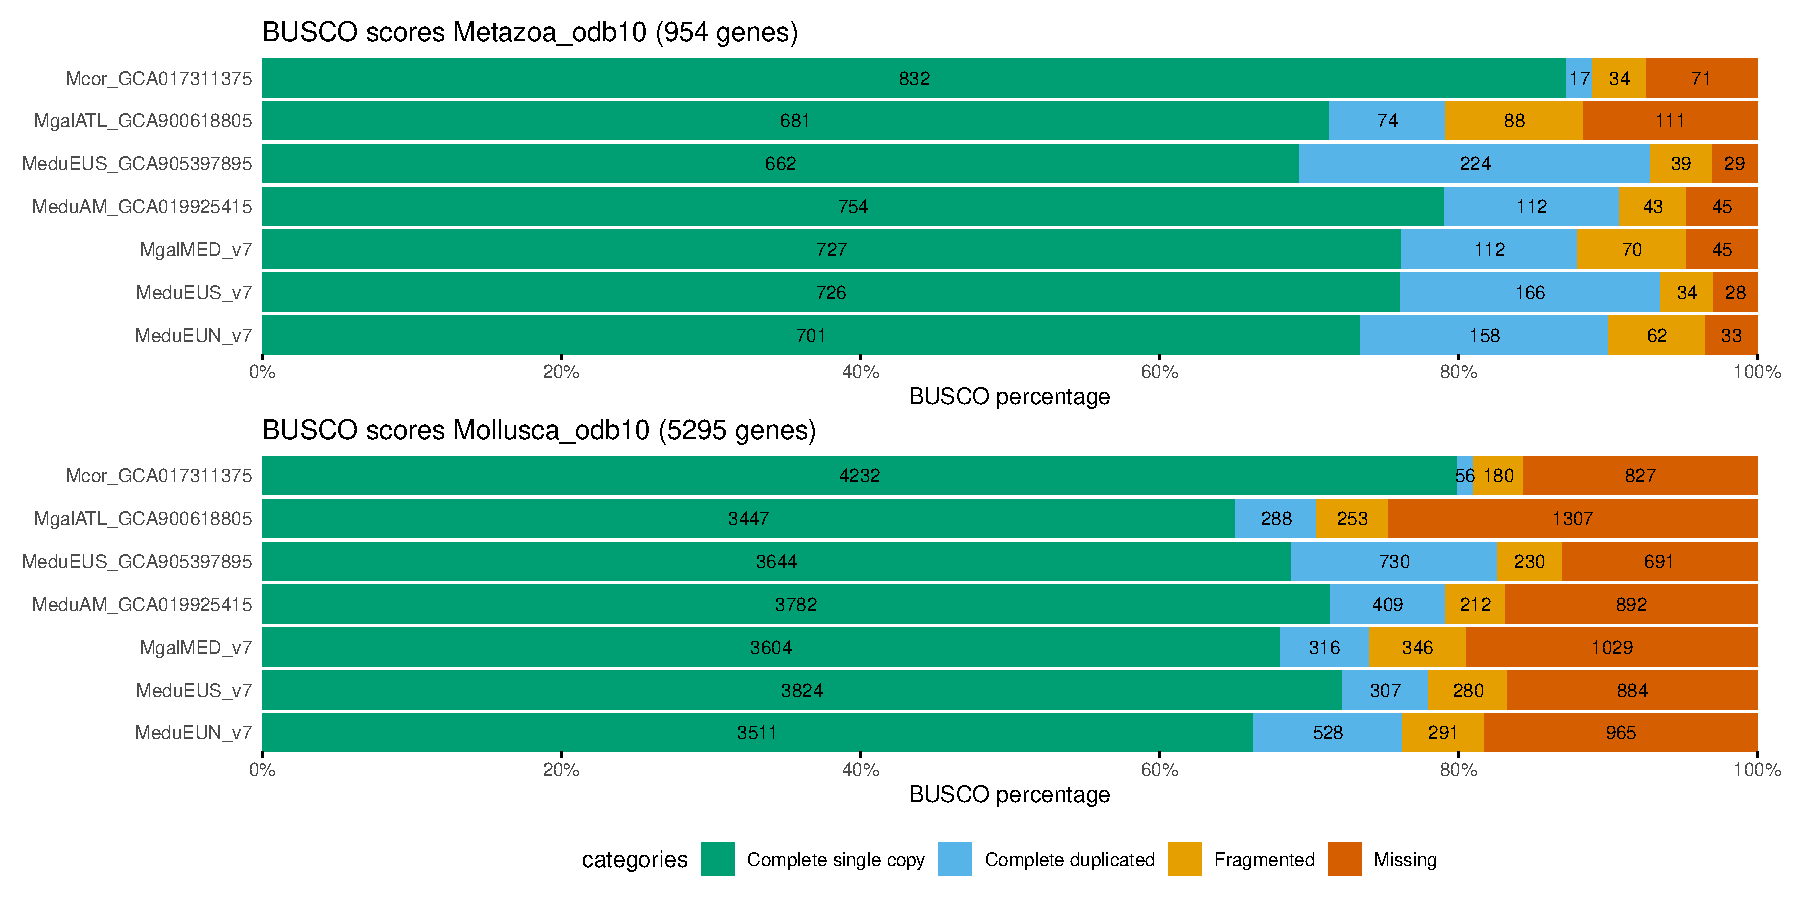
\includegraphics[width=\linewidth]{figures/Fig2_busco.pdf}
	\caption{Busco scores}
	\label{fig:busco}
\end{figure}


The species tree (\cref{fig:tree}) shows that the assemblies and the published genomes and transcriptomes are clustering as expected.
\texttt{Orthofinder} \comment{provides}{provide the orthogroups somewhere} a resource of single-copy orthogroups across a large part the \textit{Mytilus} species complex.


\begin{figure}[h]
	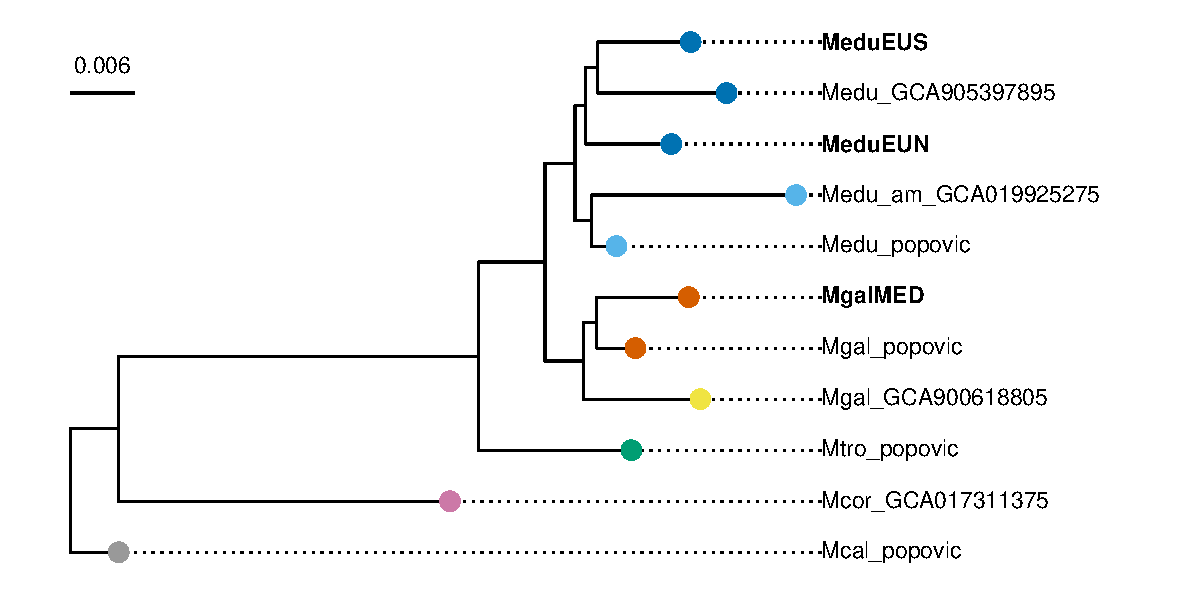
\includegraphics[width=\linewidth]{figures/Fig3_tree.pdf}
	\caption{Species tree using 1300 orthogroups with minimum of 81.8\% of species having single-copy genes in any orthogroup.
	Color coding -- dark blue: \textit{M. edulis} Europe, light blue: \textit{M. edulis} America,
	red: \textit{M. galloprovincialis} Mediterranean Sea, yellow: \textit{M. galloprovincialis} Atlantic,
	green: \textit{M. trossulus}, pink: \textit{M. coruscus}, gray: \textit{M. californianus}.
	}
	\label{fig:tree}
\end{figure}


%\includegraphics{figures/full_figure_metazoa-1.pdf}

%\section{Conclusion}\label{conclusion}


\section*{Acknowledgements}


% References
\printbibliography


%=============================================
% Supp
\newpage
\appendix
\setcounter{table}{0}
\renewcommand{\thetable}{S\arabic{table}}
\setcounter{figure}{0}
\renewcommand{\thefigure}{S\arabic{figure}}
\section*{Supplementary Information}

\subsection*{Tables}

\begin{table}[h]
	\caption{Steps carried out for each version of assembly}
	\label{suptab:versions}
	\begin{tabular}{rll}
		Version & Step & \\ \toprule
		\rowcolor{gray!20}
		v1 & Raw assembly from Supernova & \\
		v2 & Supernova assembly using a filtered dataset of reads (\cref{preproc}) & \multirow{2}{*}{\rule{1pt}{25pt} Unused} \\
		v3 & Assembly with purged duplicates (\texttt{purge\_dups}) from v3 & \\
		\rowcolor{gray!20}
		v4 & Assembly with purged duplicates (\texttt{purge\_dups}) from v1 & \\
		\rowcolor{gray!20}
		v5 & \texttt{Agouti} repaired scaffolds from v4 & \\
		\rowcolor{gray!20}
		v6 & Assembly with filtered contamination using Blobtoolkit results & \\
		\rowcolor{gray!20}
		v7 & Scaffolded assembly on \textit{M. coruscus} & \\ \bottomrule
	\end{tabular}
\end{table}
\vspace{3em}

\subsection*{Figures}
% preproc barcodes
\begin{figure}[h]
	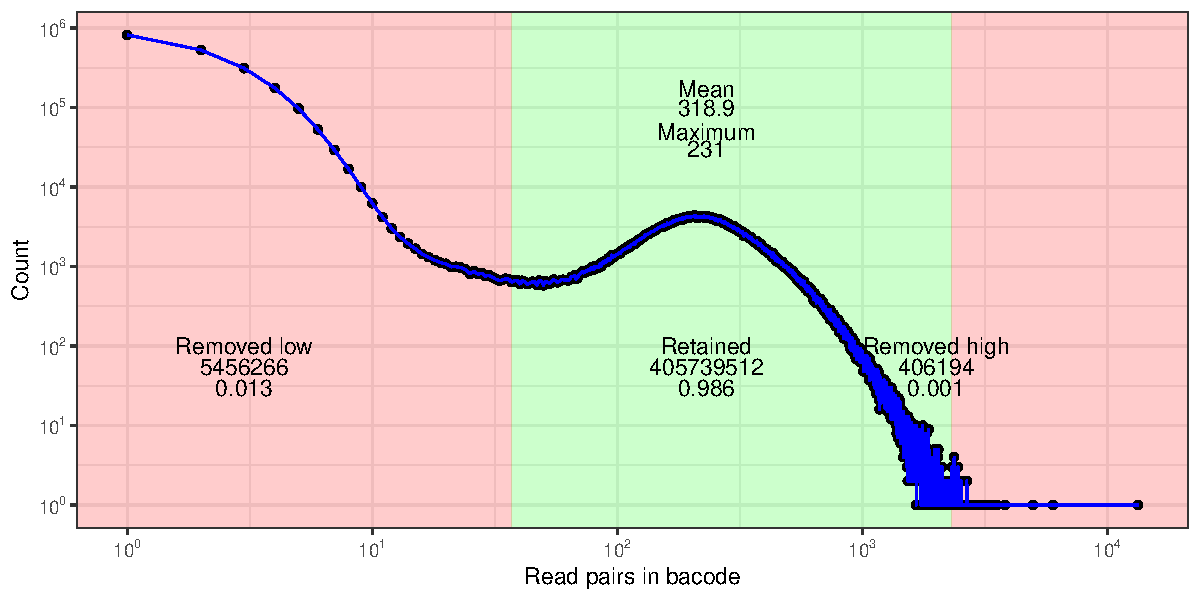
\includegraphics[width=\linewidth]{figures/MgalMED_preproc_barcode_filt.pdf}
	\caption{Histogram of read pairs identified for each 10X barcode for MgalMED.
		As part of preprocessing step, barcodes for which too few or too many read pairs are associated with each unique barcode are removed from the dataset (red regions).}
	\label{supfig:preproc_MgalMED}
\end{figure}

\begin{figure}[h]
	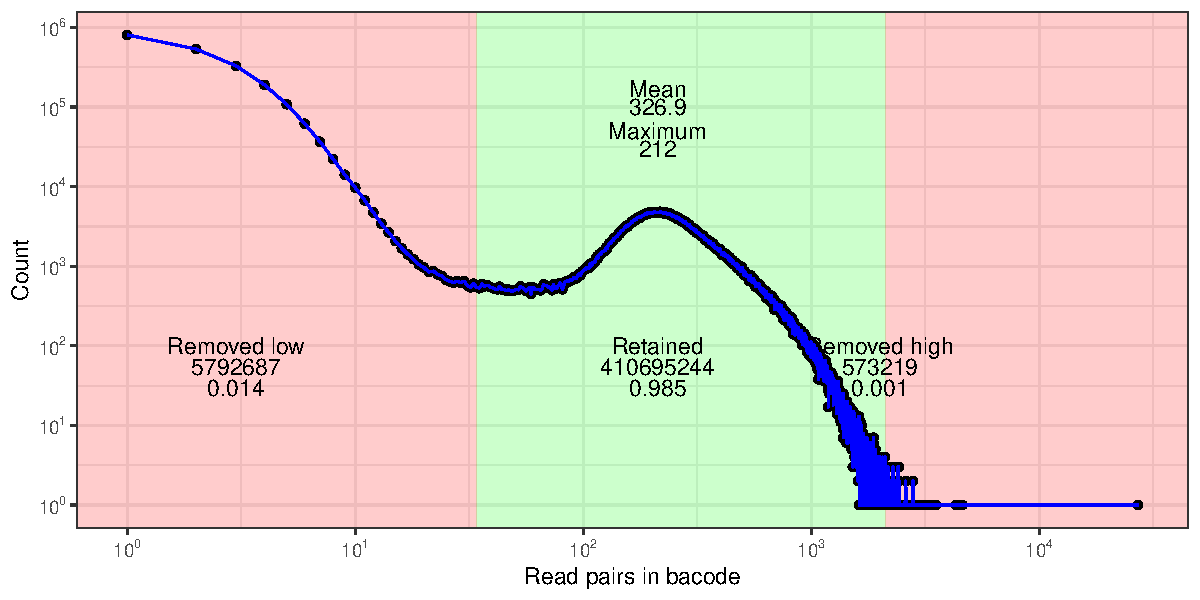
\includegraphics[width=\linewidth]{figures/MeduEUS_preproc_barcode_filt.pdf}
	\caption{Histogram of read pairs identified for each 10X barcode for MeduEUS.
		As part of preprocessing step, barcodes for which too few or too many read pairs are associated with each unique barcode are removed from the dataset (red regions).}
	\label{supfig:preproc_MeduEUS}
\end{figure}

\begin{figure}[h]
	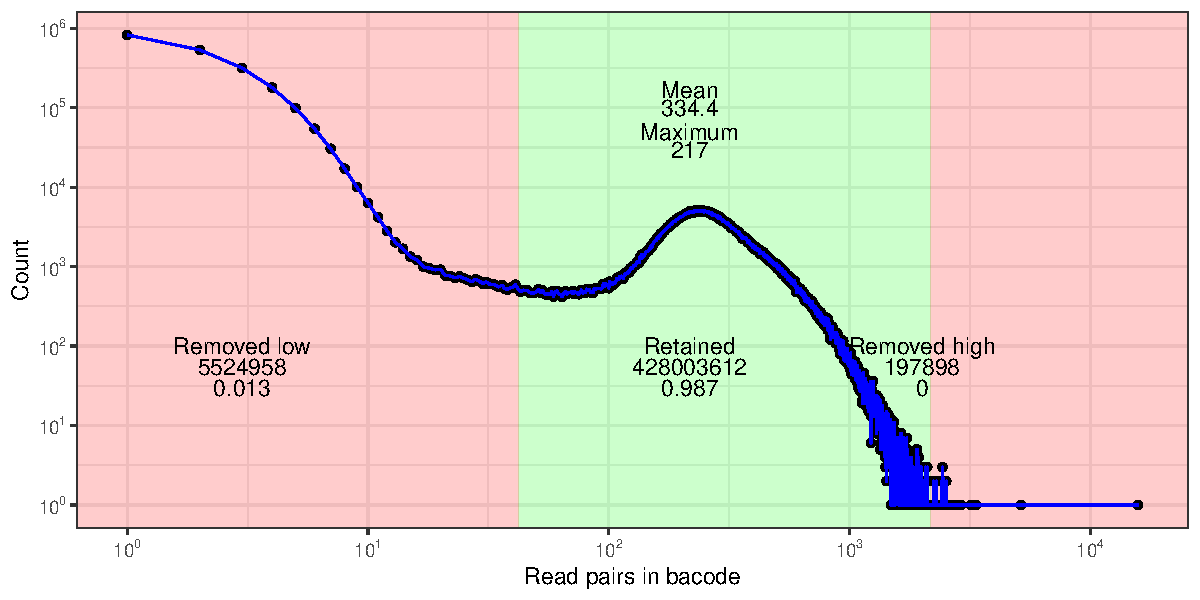
\includegraphics[width=\linewidth]{figures/MeduEUN_preproc_barcode_filt.pdf}
	\caption{Histogram of read pairs identified for each 10X barcode for MeduEUN.
	As part of preprocessing step, barcodes for which too few or too many read pairs are associated with each unique barcode are removed from the dataset (red regions).}
	\label{supfig:preproc_MeduEUN}
\end{figure}

\begin{figure}[h]
	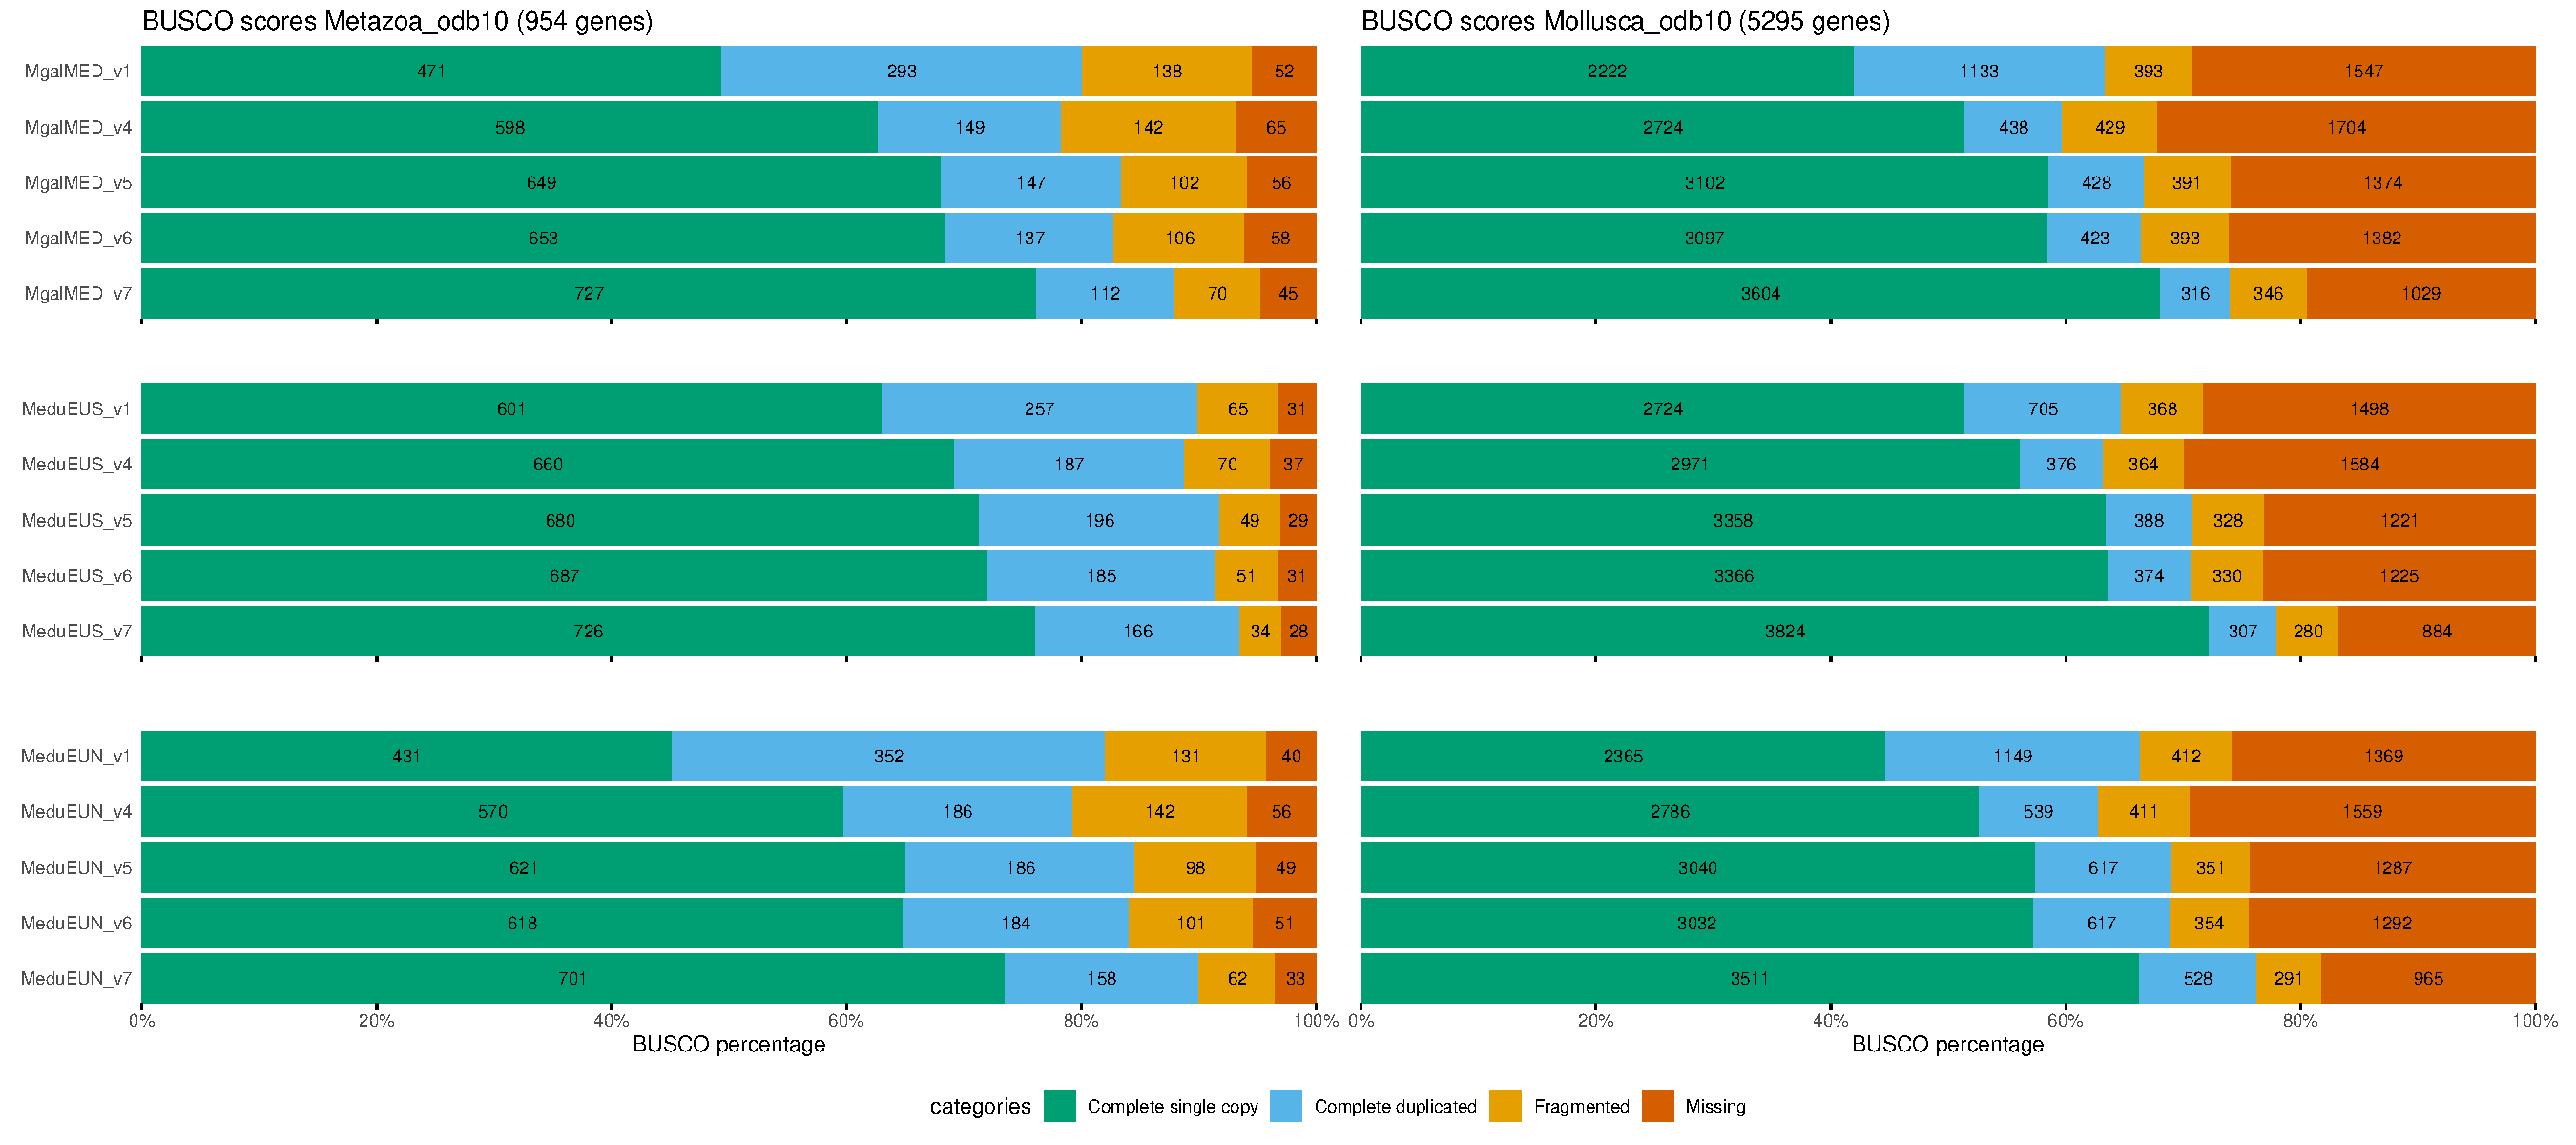
\includegraphics[width=\linewidth]{figures/supfig_busco.pdf}
	\caption{Busco scores on the metazoa\_odb10 (left panels) and mollusca\_odb10 (right panels) databases for each assembly MgalMED, MeduEUS and MeduEUN (top to bottom panels) across several assembly versions (v1, v4, v5, v6, v7).}
	\label{supfig:busco}
\end{figure}

% blobs
\begin{figure}
	\includegraphics[width=\linewidth]{figures/btk_blob_MgalMED_v7}
	\caption{Blobtoolkit blob plot of base coverage in GM against GC proportion for scaffolds in assembly MgalMED\_v7. Scaffolds are colored by phylum and binned at a resolution of 30 divisions on each axis. Colored squares within each bin are sized in proportion to the sum of individual scaffold lengths on a square-root scale, ranging from 1,005 to 1,127,105,406. Histograms show the distribution of scaffold length sum along each axis.}
	\label{supfig:btk-blob-MgalMED}
\end{figure}

\begin{figure}
	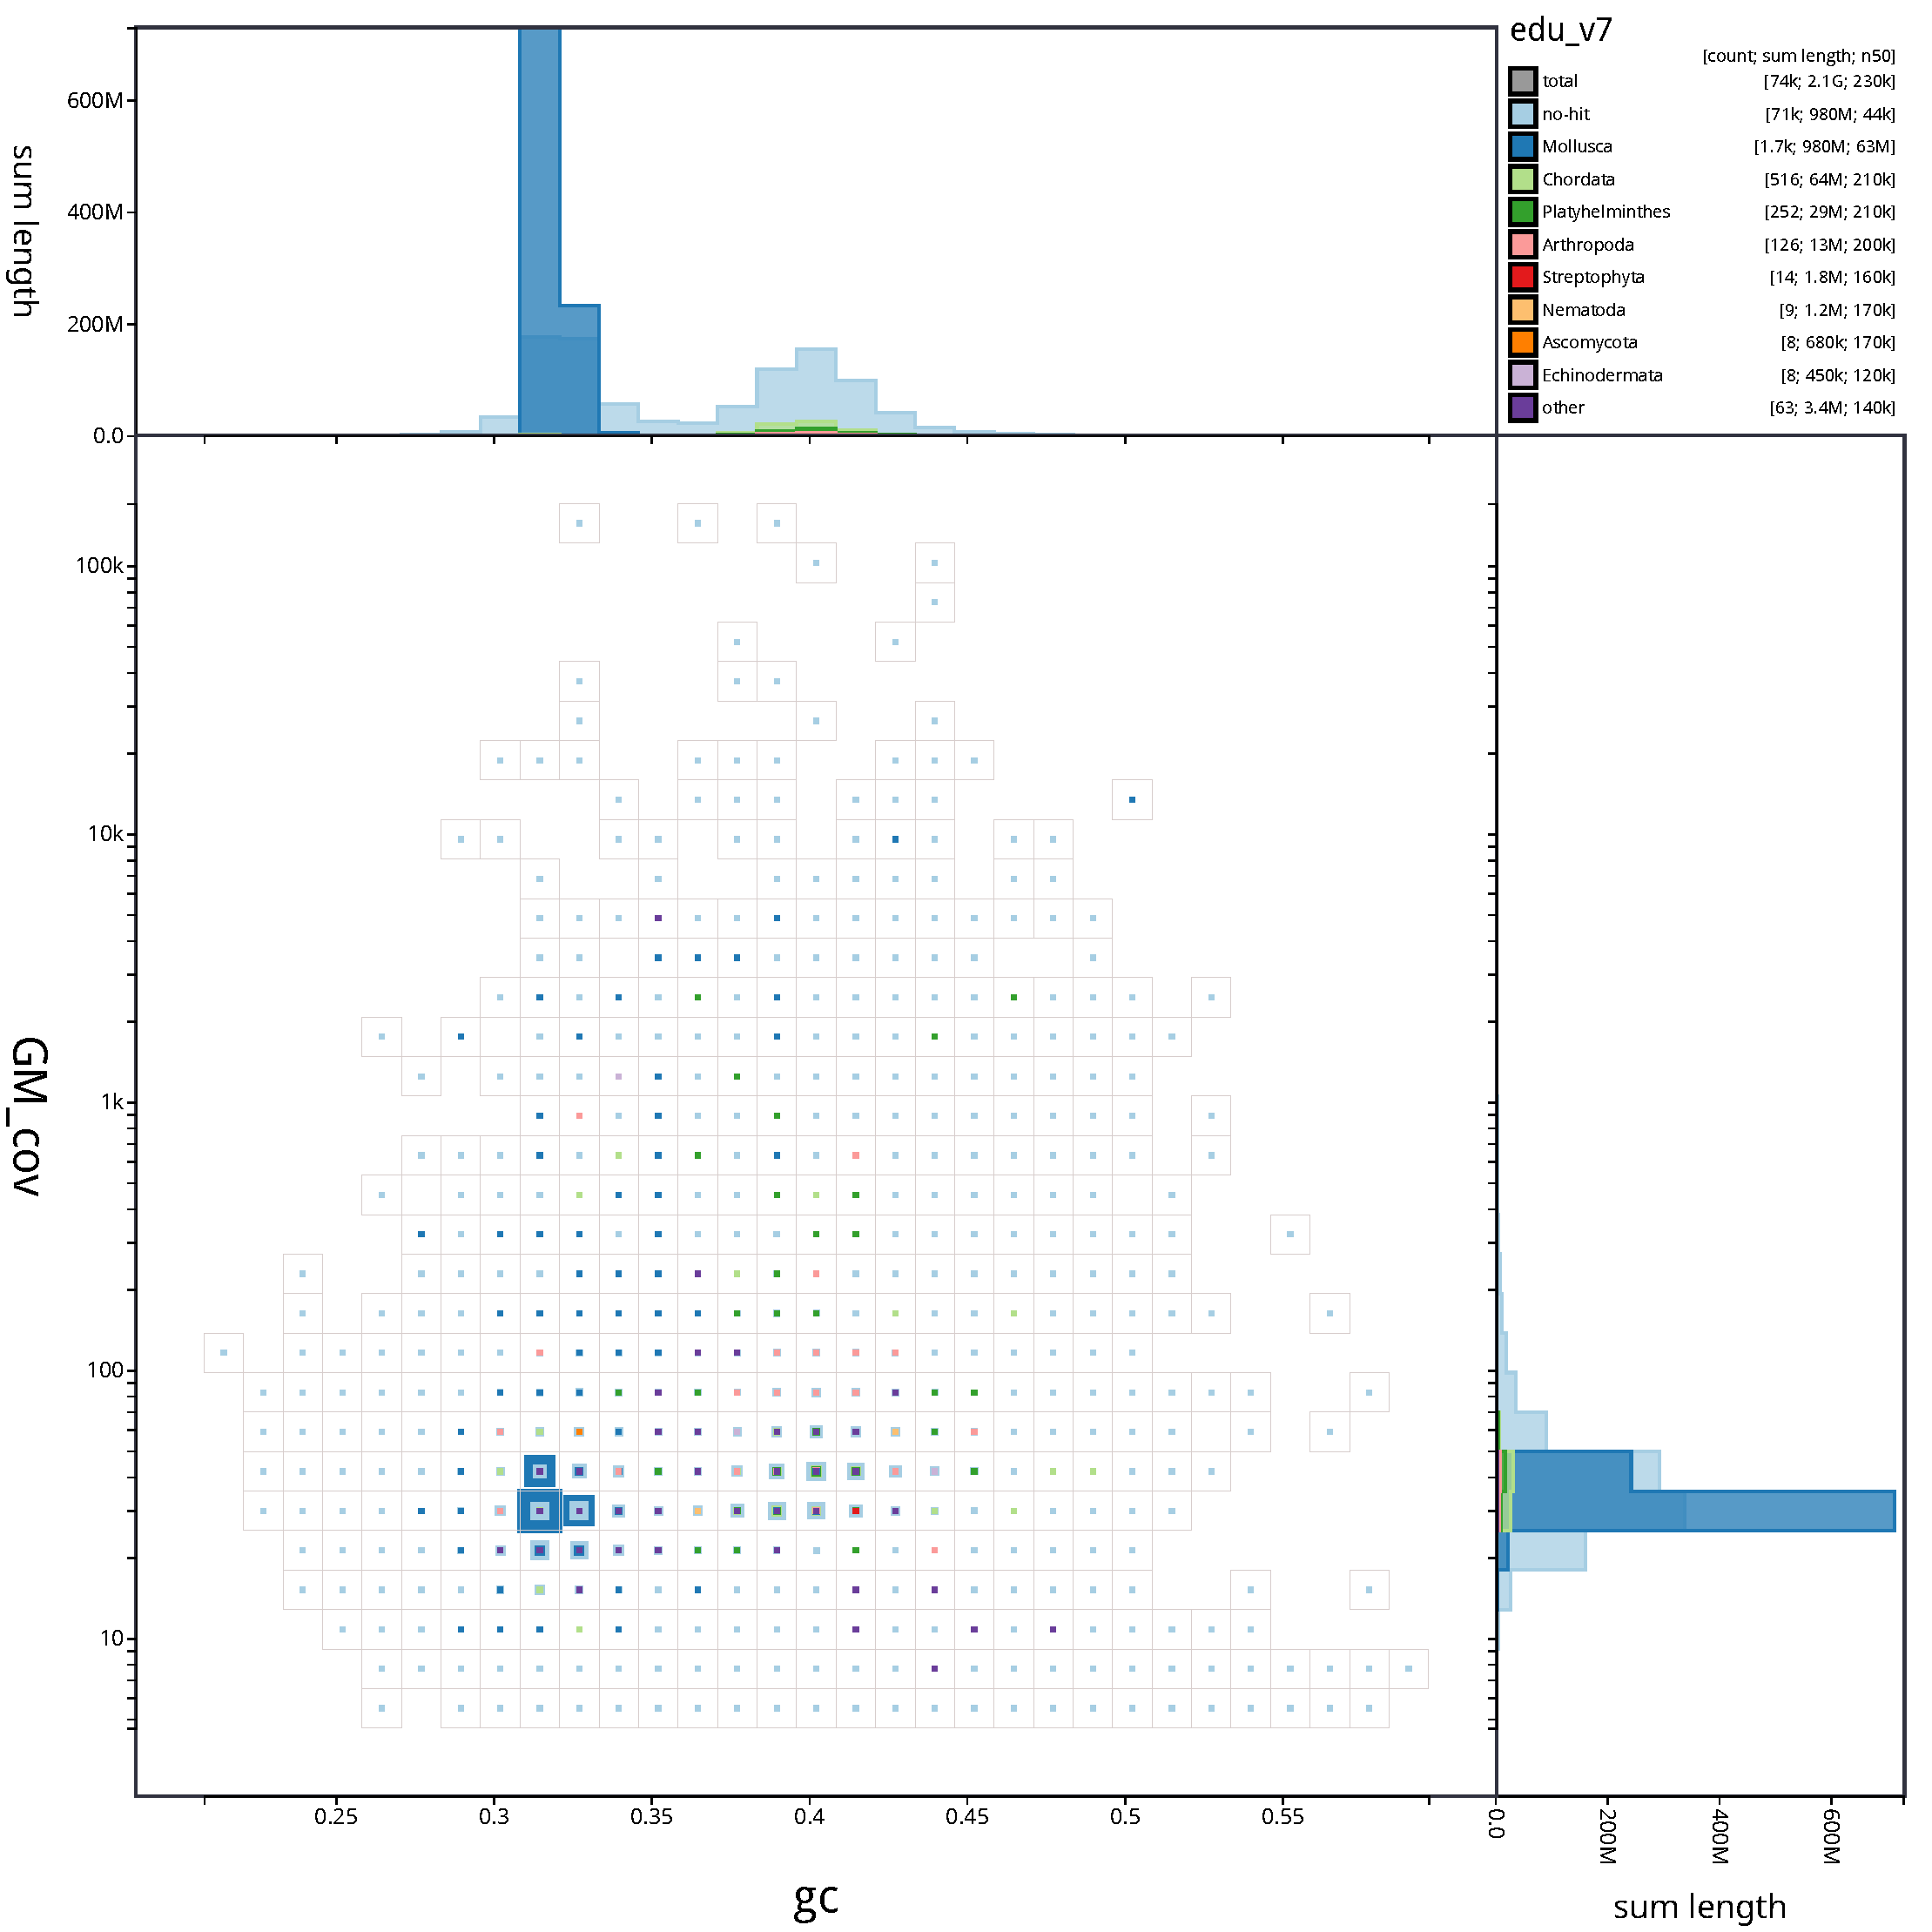
\includegraphics[width=\linewidth]{figures/btk_blob_MeduEUS_v7}
	\caption{Blobtoolkit blob plot of base coverage in GM against GC proportion for scaffolds in assembly MeduEUS\_v7. Scaffolds are colored by phylum and binned at a resolution of 30 divisions on each axis. Colored squares within each bin are sized in proportion to the sum of individual scaffold lengths on a square-root scale, ranging from 987 to 487,517,891. Histograms show the distribution of scaffold length sum along each axis.}
	\label{supfig:btk-blob-MeduEUS}
\end{figure}

\begin{figure}
	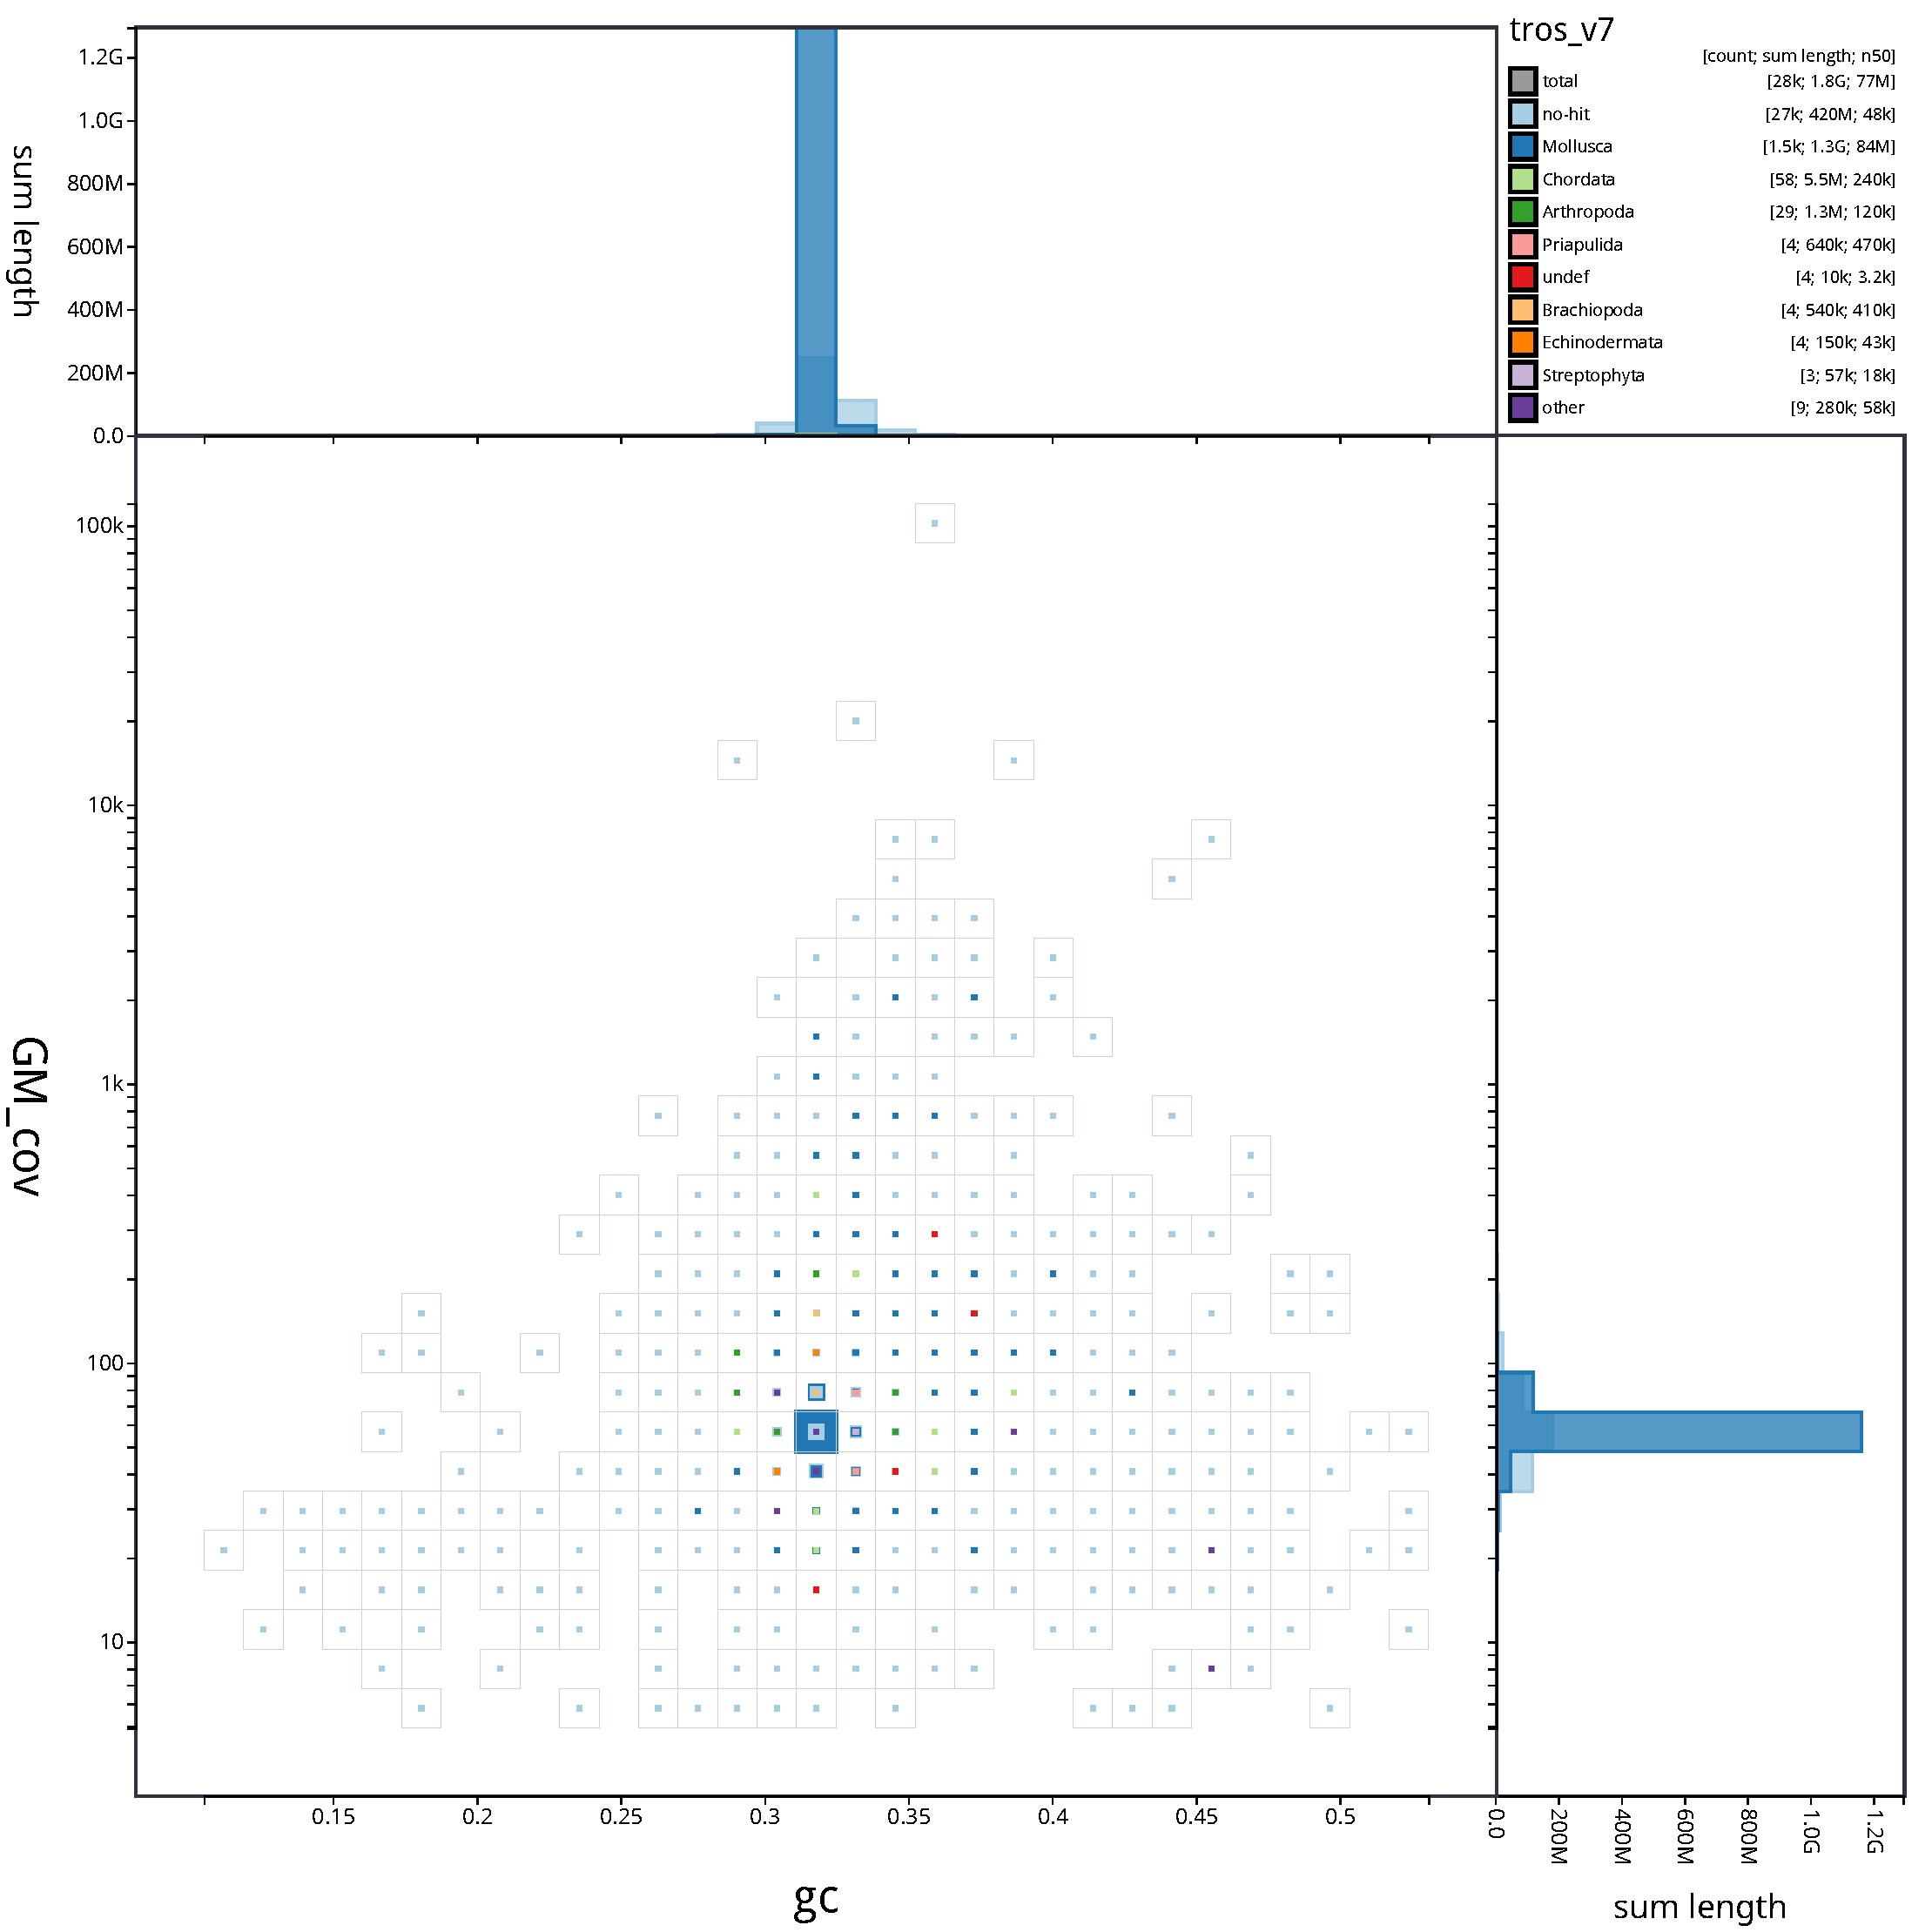
\includegraphics[width=\linewidth]{figures/btk_blob_MeduEUN_v7}
	\caption{Blobtoolkit blob plot of base coverage in GM against GC proportion for scaffolds in assembly MeduEUN\_v7. Scaffolds are colored by phylum and binned at a resolution of 30 divisions on each axis. Colored squares within each bin are sized in proportion to the sum of individual scaffold lengths on a square-root scale, ranging from 1,011 to 1,136,301,196. Histograms show the distribution of scaffold length sum along each axis.}
	\label{supfig:btk-blob-MeduEUN}
\end{figure}

% cumulative lengths
\begin{figure}
	\includegraphics[width=\linewidth]{figures/btk_cumulative_MgalMED_v7}
	\caption{Blobtoolkit cumulative scaffold length for assembly MgalMED\_v7. The gray line shows cumulative length for all scaffolds. Colored lines show cumulative lengths of scaffolds assigned to each phylum using the bestsumorder taxrule.}
	\label{supfig:btk-cumul-MgalMED}
\end{figure}

\begin{figure}
	\includegraphics[width=\linewidth]{figures/btk_cumulative_MeduEUS_v7}
	\caption{Blobtoolkit cumulative scaffold length for assembly MeduEUS\_v7. The gray line shows cumulative length for all scaffolds. Colored lines show cumulative lengths of scaffolds assigned to each phylum using the bestsumorder taxrule.}
	\label{supfig:btk-cumul-MeduEUS}
\end{figure}

\begin{figure}
	\includegraphics[width=\linewidth]{figures/btk_cumulative_MeduEUN_v7}
	\caption{Blobtoolkit cumulative scaffold length for assembly MeduEUN\_v7. The gray line shows cumulative length for all scaffolds. Colored lines show cumulative lengths of scaffolds assigned to each phylum using the bestsumorder taxrule.}
	\label{supfig:btk-cumul-MeduEUN}
\end{figure}

% snail plots
\begin{figure}
	\includegraphics[width=\linewidth]{figures/btk_snail_MgalMED_v7}
	\caption{Blobtoolkit snail plot summary of assembly statistics for assembly MgalMED\_v7. The main plot is divided into 1,000 size-ordered bins around the circumference with each bin representing 0.1\% of the 1,658,656,017 bp assembly. The distribution of scaffold lengths is shown in dark gray with the plot radius scaled to the longest scaffold present in the assembly (104,729,878 bp, shown in red). Orange and pale-orange arcs show the N50 and N90 scaffold lengths (71,952,646 and 16,011 bp), respectively. The pale gray spiral shows the cumulative scaffold count on a log scale with white scale lines showing successive orders of magnitude. The blue and pale-blue area around the outside of the plot shows the distribution of GC, AT and N percentages in the same bins as the inner plot. A summary of complete, fragmented, duplicated and missing BUSCO genes in the mollusca\_odb10 set is shown in the top right.}
	\label{supfig:btk-snail-MgalMED}
\end{figure}

\begin{figure}
	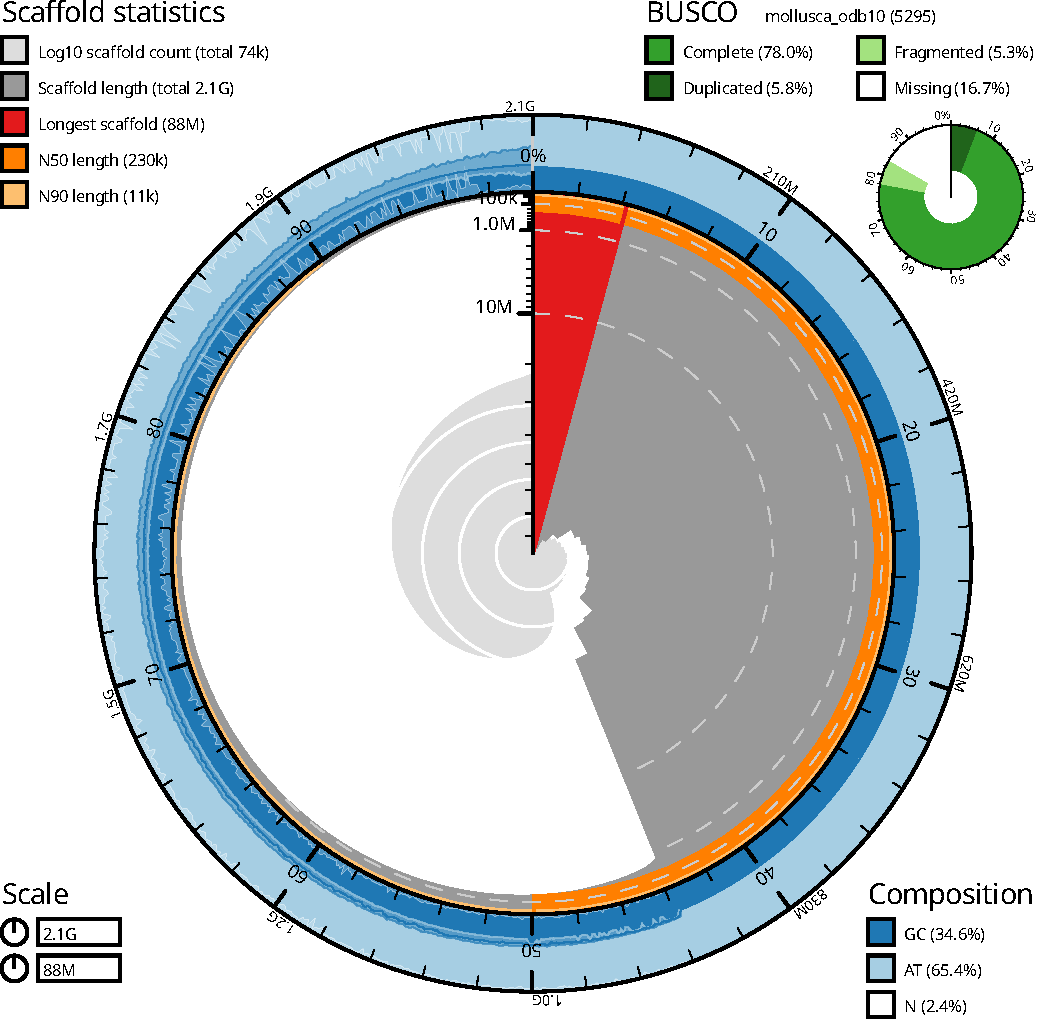
\includegraphics[width=\linewidth]{figures/btk_snail_MeduEUS_v7}
	\caption{Blobtoolkit snail plot summary of assembly statistics for assembly MeduEUS\_v7. The main plot is divided into 1,000 size-ordered bins around the circumference with each bin representing 0.1\% of the 2,076,685,641 bp assembly. The distribution of scaffold lengths is shown in dark gray with the plot radius scaled to the longest scaffold present in the assembly (88,305,666 bp, shown in red). Orange and pale-orange arcs show the N50 and N90 scaffold lengths (228,263 and 10,773 bp), respectively. The pale gray spiral shows the cumulative scaffold count on a log scale with white scale lines showing successive orders of magnitude. The blue and pale-blue area around the outside of the plot shows the distribution of GC, AT and N percentages in the same bins as the inner plot. A summary of complete, fragmented, duplicated and missing BUSCO genes in the mollusca\_odb10 set is shown in the top right. }
	\label{supfig:btk-snail-MeduEUS}
\end{figure}

\begin{figure}
	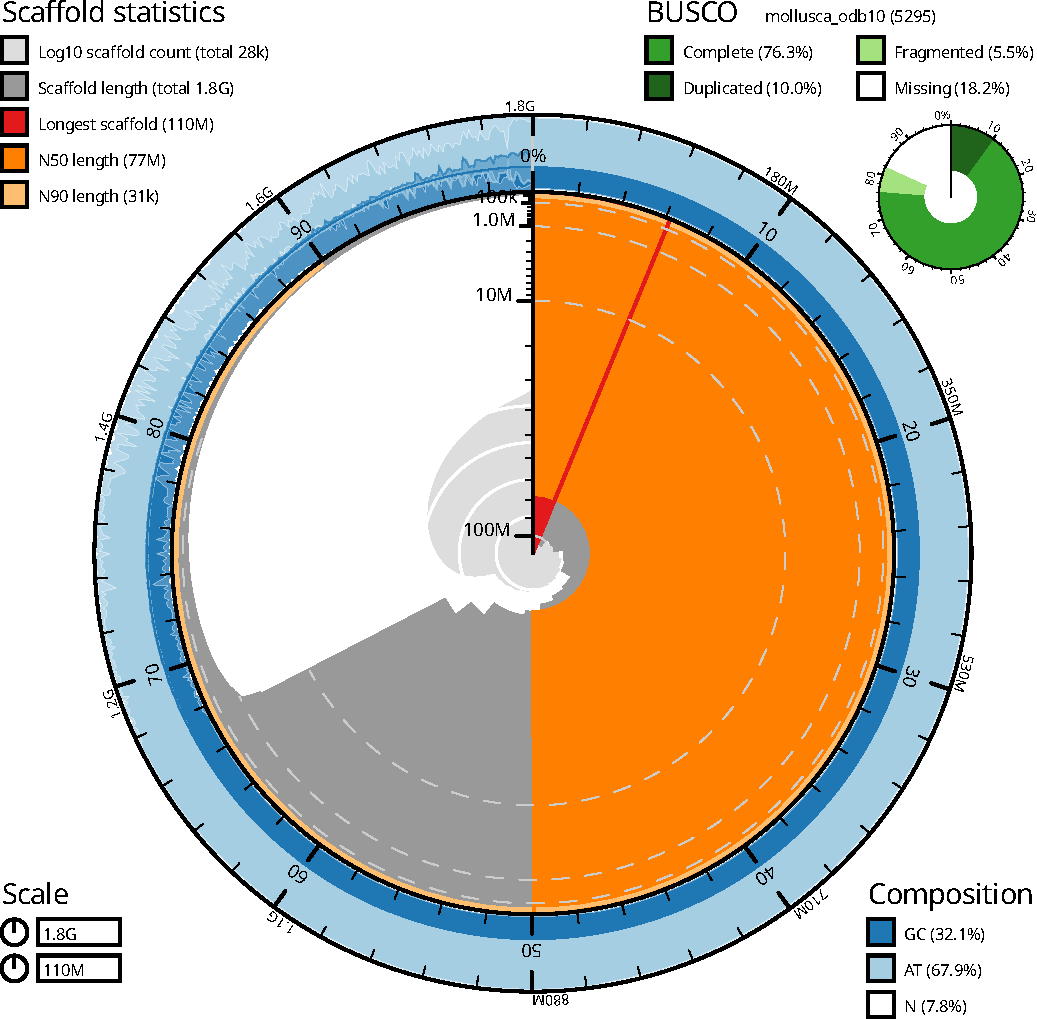
\includegraphics[width=\linewidth]{figures/btk_snail_MeduEUN_v7}
	\caption{Blobtoolkit snail plot summary of assembly statistics for assembly MeduEUN\_v7. The main plot is divided into 1,000 size-ordered bins around the circumference with each bin representing 0.1\% of the 1,764,246,486 bp assembly. The distribution of scaffold lengths is shown in dark gray with the plot radius scaled to the longest scaffold present in the assembly (110,194,685 bp, shown in red). Orange and pale-orange arcs show the N50 and N90 scaffold lengths (77,102,752 and 30,649 bp), respectively. The pale gray spiral shows the cumulative scaffold count on a log scale with white scale lines showing successive orders of magnitude. The blue and pale-blue area around the outside of the plot shows the distribution of GC, AT and N percentages in the same bins as the inner plot. A summary of complete, fragmented, duplicated and missing BUSCO genes in the mollusca\_odb10 set is shown in the top right.}
	\label{supfig:btk-snail-MeduEUN}
\end{figure}

\end{document}
